\documentclass[conference]{IEEEtran}
\usepackage{array}
\usepackage[caption=true,font=footnotesize,labelfont=rm,textfont=rm]{subfig}
\usepackage{textcomp}
\usepackage{stfloats}
\usepackage{url}
\usepackage{verbatim}
\usepackage{graphicx}
\usepackage{tikz}
\usetikzlibrary{arrows.meta,positioning,fit,calc,backgrounds,shapes.geometric}
\hyphenation{op-tical net-works semi-conduc-tor IEEE-Xplore}
\def\BibTeX{{\rm B\kern-.05em{\sc i\kern-.025em b}\kern-.08em
    T\kern-.1667em\lower.7ex\hbox{E}\kern-.125emX}}
\usepackage{balance}

\usepackage{amssymb,amsfonts}
\usepackage[tbtags]{amsmath}

\usepackage[ruled,linesnumbered]{algorithm2e}
\usepackage{color}
\usepackage{booktabs}
\usepackage[thmmarks,amsmath]{ntheorem}
\usepackage{setspace}
\usepackage{hyperref}
\usepackage{cite}
\usepackage{soul}
\soulregister{\cite}7
\captionsetup{font={footnotesize}}
{
    \theoremstyle{nonumberplain}
    \theoremheaderfont{\bfseries\itshape}
    \theorembodyfont{\normalfont}
    \theoremseparator{:}
    \theoremsymbol{\ensuremath{\blacksquare}}
    \newtheorem{proof}{Proof}
}
{
    \theoremstyle{plain}
    \theoremheaderfont{\bfseries\itshape}
    \theorembodyfont{\normalfont}
    \theoremseparator{:}
    \theoremsymbol{\ensuremath{\blacksquare}}
    \newtheorem{remark}{Remark}
    \newtheorem{definition}{Definition}
    \newtheorem{lemma}{Lemma}
    \newtheorem{theorem}{Theorem}
}

\newcommand{\algref}[1]{\textit{\textbf{Algorithm \ref{#1}}}}
\newcommand{\theoref}[1]{\textit{\textbf{Theorem \ref{#1}}}}
\newcommand{\lemmref}[1]{\textit{\textbf{Lemma \ref{#1}}}}
\newcommand{\defref}[1]{\textit{\textbf{Definition \ref{#1}}}}
\newcommand{\figref}[1]{Fig. \ref{#1}}
\providecommand{\resultfigdir}{figures}
\providecommand{\methodfigdir}{figures}
\pdfoutput=1

\begin{document}

\title{Guided-DiffFNO: Critic-Guided Diffusion Policy for IoT-Enabled Multi-Zone Building HVAC Control}

\author{Wei Zou, Yu Sun, Haibo Zhou,~\IEEEmembership{Fellow,~IEEE}}

\maketitle

\begin{abstract}
IoT sensor networks enable real-time thermal monitoring and control command delivery, making data-driven HVAC optimization promising for building energy management. However, multi-zone HVAC control remains difficult for standard reinforcement learning policies because actions are coupled across zones, unimodal policies are restrictive, and MLP backbones do not explicitly model zone-wise coordination. This paper presents Guided-DiffFNO, a generative controller for IoT-enabled multi-zone HVAC systems. It combines a conditional diffusion policy, an FNO denoiser over the action-dimension axis, and inference-time double-critic guidance. Experiments on the BEAR OfficeSmall-Hot\_Dry benchmark show that Guided-DiffFNO achieves the lowest comfort violations and the best test reward among the learned controllers considered, while producing smoother and more spectrally regular control signals than unguided diffusion and the MLP-denoiser baseline.
\end{abstract}

\begin{IEEEkeywords}
IoT-enabled buildings, HVAC control, diffusion policy, Fourier neural operator, critic guidance, reinforcement learning.
\end{IEEEkeywords}

\section{Introduction}

Buildings account for a substantial portion of global energy consumption, and HVAC systems are among the largest controllable contributors to operational energy use \cite{perez2008review,cao2016building,cuce2026role}. In IoT-enabled buildings, distributed sensors continuously monitor zone temperatures, outdoor conditions, solar irradiance, and occupancy-related loads. These measurements are aggregated through gateway nodes and fed into the control policy at each decision step. The resulting control actions are then applied to zone-level HVAC actuators through the same IoT infrastructure, closing the sensing--actuation loop. This closed-loop digital infrastructure makes data-driven HVAC control increasingly relevant for large commercial buildings.

Recent RL approaches provide a model-free alternative to rule-based control and model predictive control (MPC), but standard policies remain mismatched to multi-zone HVAC control in three ways \cite{drgovna2020all,wei2017deep,biemann2021experimental,mason2019review,alsayed2024hvacreview}. First, many continuous-control methods use deterministic mappings or unimodal Gaussian action distributions, which are too restrictive when multiple coordinated control patterns are feasible under the same thermal state. Second, common multilayer perceptron (MLP) backbones do not explicitly encode cross-zone coupling and therefore struggle to capture the structured geometry of the joint action vector. Third, unguided policies often generate oscillatory actions, which may increase energy use, reduce comfort, and lead to less regular operation in coupled building systems.

Diffusion policies offer a more expressive action model for continuous control \cite{chi2025diffusion,janner2022planning,wang2023diffusion}, while Fourier Neural Operators (FNOs) provide a useful spectral prior when dominant low-frequency coordination is desired \cite{li2021fourier,qin2024toward,liu2024mitigating}. Motivated by these observations, we formulate the multi-zone HVAC policy as a conditional reverse-diffusion process and replace the standard MLP denoiser with an FNO backbone that acts directly on the action-dimension axis. We then refine reverse sampling with gradients from a conservative double critic so that the policy is both distributionally expressive and value-aware during inference.
The action-dimension axis can be viewed as a compact control field over thermal zones: neighboring or strongly coupled zones should generally receive coordinated commands, whereas abrupt high-frequency variation across action coordinates often indicates inefficient or implausible control. This view is well aligned with networked building automation, where decisions are made from synchronized multi-zone measurements rather than isolated room observations. The policy class should therefore represent multiple feasible joint actions, preserve cross-zone consistency, and remain stable under repeated sensor-driven updates.

This formulation differs from two related lines of work. Unlike conventional building RL, the policy is not treated as a point estimator over each action coordinate; instead, the full multi-zone command is modeled as a generated object. Unlike generic diffusion control, building-specific structure is introduced through spectral action modeling and critic-guided refinement. This combination tailors Guided-DiffFNO to centralized IoT-enabled HVAC control rather than directly applying a generic diffusion policy. In particular, once IoT sensing aggregates building-wide measurements into a common state vector, the controller must map that shared state to a coordinated joint action, which directly motivates a state-conditional generative policy with explicit action-space structure.

The main contributions of this paper are:
\begin{itemize}
    \item We propose \emph{Guided-DiffFNO}, an IoT-oriented generative HVAC controller that models the full joint zone action through conditional diffusion rather than point-estimate regression.
    \item We introduce a DiffFNO denoiser that imposes a spectral inductive bias over the action-dimension axis, improving cross-zone coordination and suppressing high-frequency control chatter.
    \item We design an inference-time critic-guidance mechanism and show on the BEAR benchmark that it improves the overall energy--comfort balance over unguided diffusion and the MLP-denoiser baseline.
\end{itemize}

The remainder of this paper is organized as follows. Section~\ref{sec:system_model} introduces the IoT-enabled multi-zone HVAC control setting and the MDP formulation. Section~\ref{sec:method} presents Guided-DiffFNO, including the conditional diffusion policy, DiffFNO backbone, critic guidance, and training framework. Section~\ref{sec:experiments} reports the experimental setup and results, and Section~\ref{sec:conclusion} concludes the paper.

\section{System Model}
\label{sec:system_model}

\begin{figure}[!t]
    \captionsetup{width=\linewidth}
    \centerline{\includegraphics[width=\linewidth]{figures/Control Architecture.pdf}}
    \caption{IoT-enabled sensing--control architecture for multi-zone building HVAC control. Zone-level measurements are gathered by the gateway node, aggregated into the state vector $\mathbf{s}_t$, and fed to the control policy, whose joint action is applied back to the building.}
    \label{fig:system_model}
\end{figure}

Figure~\ref{fig:system_model} illustrates the closed-loop IoT architecture considered in this paper. Zone-level sensing data are gathered through the gateway node, passed through the building data layer, and aggregated into the state vector $\mathbf{s}_t$ used by the policy. The resulting joint control action is then applied to the zone-level HVAC actuators.
We formulate multi-zone HVAC control as a discounted MDP $\mathcal{M}=(\mathcal{S},\mathcal{A},\mathcal{P},r,\gamma)$, where the transition kernel is induced by the physics-based BEAR simulator \cite{zhang2023bear}. The controller interacts with a six-zone office building under coupled thermal dynamics, weather disturbances, solar gains, and internal loads.
The state vector $\mathbf{s}_t$ is constructed from aggregated IoT measurements collected across all thermal zones, including zone temperatures, outdoor temperature, solar irradiance, ground temperature, and internal loads. Figure~\ref{fig:system_model} highlights representative components of $\mathbf{s}_t$, while the ellipsis denotes additional exogenous features such as the ground-temperature term. The action is a continuous joint HVAC command for all $N$ zones:
\begin{equation}
    \mathbf{a}_t =
    [a_{t,1}, a_{t,2}, \dots, a_{t,N}]
    \in [-1,1]^N,
    \label{eq:action}
\end{equation}
Consequently, the policy must generate a coordinated multi-zone control vector rather than independent per-zone decisions. Because the six zones share disturbances and thermal interactions, a command that appears locally beneficial for one zone may still be globally inefficient once neighboring temperatures, comfort violations, and total HVAC energy are considered jointly.

The reward combines the simulator reward with an explicit thermal-comfort violation penalty:
\begin{equation}
    d_{t,i}=\left|T_{t,i}^{\mathrm{zone}}-T^{\mathrm{ref}}\right|,
    \qquad
    V_t=\sum_{i=1}^{N}\mathbb{I}(d_{t,i}>\delta),
    \label{eq:violation}
\end{equation}
\begin{equation}
    r_t = \rho \left( r_t^{\mathrm{env}} - \lambda V_t \right),
    \label{eq:reward}
\end{equation}
where $T^{\mathrm{ref}}$ is the target temperature, $\delta$ is the comfort tolerance, $V_t$ counts zone-wise temperature violations with respect to the comfort band defined by ASHRAE Standard 55 \cite{standard2023thermal}, $\lambda$ is the violation penalty, and $\rho$ is a reward-scaling coefficient. The control objective is
\begin{equation}
    J(\pi)=\mathbb{E}_{\pi}\left[\sum_{t=0}^{T-1}\gamma^t r_t\right].
    \label{eq:objective}
\end{equation}
This objective captures the control goal of reducing HVAC energy while avoiding persistent comfort-band violations across the monitored thermal zones.

\section{Guided-DiffFNO Method}
\label{sec:method}

\subsection{Conditional Diffusion Policy}

Instead of regressing a single action from $\mathbf{s}_t$, we generate actions through a conditional denoising process \cite{ho2020denoising}. In the IoT-enabled control loop considered in this paper, $\mathbf{s}_t$ is the aggregated building state formed from synchronized sensor measurements across zones, and the generated action is dispatched back to the HVAC actuators through the same supervisory infrastructure. Let $\mathbf{x}_0$ denote the clean action and $\mathbf{x}_k$ its noisy version at reverse step $k$. Under the variance-preserving parameterization,
\begin{equation}
    \mathbf{x}_k =
    \sqrt{\bar{\alpha}_k}\mathbf{x}_0 +
    \sqrt{1-\bar{\alpha}_k}\boldsymbol{\epsilon},
    \qquad
    \boldsymbol{\epsilon}\sim\mathcal{N}(\mathbf{0},\mathbf{I}),
    \label{eq:noisy_action}
\end{equation}
and the denoiser directly predicts the clean action
\begin{equation}
    \hat{\mathbf{x}}_0 = f_{\theta}(\mathbf{x}_k, k, \mathbf{s}_t).
    \label{eq:x0_prediction}
\end{equation}
Under the standard DDPM parameterization, the reverse posterior mean can be written as
\begin{equation}
    \boldsymbol{\mu}_k(\hat{\mathbf{x}}_0,\mathbf{x}_k)=
    c_1(k)\hat{\mathbf{x}}_0 + c_2(k)\mathbf{x}_k,
    \label{eq:posterior_mean}
\end{equation}
where $c_1(k)$ and $c_2(k)$ are determined by the noise schedule. Starting from Gaussian noise, the policy iteratively reconstructs a feasible multi-zone action through reverse DDPM sampling. This formulation is attractive for HVAC control because it can represent richer action distributions than deterministic or unimodal Gaussian policies and also provides a natural interface for structural and value-based guidance.

\begin{figure*}[!t]
    \centering
    \IfFileExists{\methodfigdir/guided_difffno_framework.pdf}{
        \includegraphics[width=\textwidth]{\methodfigdir/guided_difffno_framework.pdf}
    }{
        \resizebox{\textwidth}{!}{
        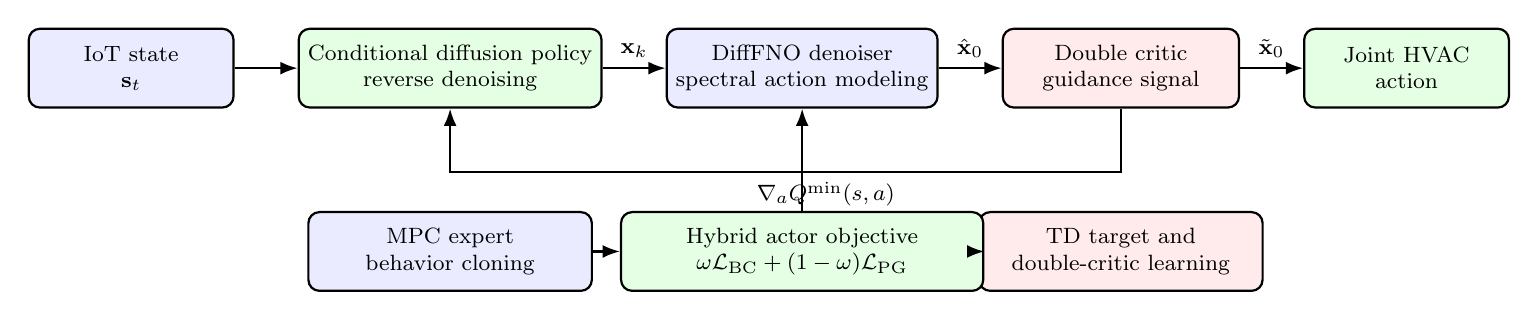
\begin{tikzpicture}[
            font=\footnotesize,
            node distance=6mm and 8mm,
            box/.style={draw, rounded corners, thick, align=center, minimum height=10mm, minimum width=28mm, fill=blue!8},
            mid/.style={draw, rounded corners, thick, align=center, minimum height=10mm, minimum width=24mm, fill=green!10},
            crit/.style={draw, rounded corners, thick, align=center, minimum height=10mm, minimum width=24mm, fill=red!8},
            arrow/.style={-{Latex[length=2.2mm]}, thick}
        ]
            \node[box, minimum width=26mm] (state) {IoT state\\$\mathbf{s}_t$};
            \node[mid, right=8mm of state, minimum width=36mm] (diff) {Conditional diffusion policy\\reverse denoising};
            \node[box, right=8mm of diff, minimum width=34mm] (fno) {DiffFNO denoiser\\spectral action modeling};
            \node[crit, right=8mm of fno, minimum width=30mm] (critic) {Double critic\\guidance signal};
            \node[mid, right=8mm of critic, minimum width=26mm] (action) {Joint HVAC\\action};

            \draw[arrow] (state) -- (diff);
            \draw[arrow] (diff) -- node[above] {$\mathbf{x}_k$} (fno);
            \draw[arrow] (fno) -- node[above] {$\hat{\mathbf{x}}_0$} (critic);
            \draw[arrow] (critic) -- node[above] {$\tilde{\mathbf{x}}_0$} (action);
            \draw[arrow] (critic.south) |- ++(0,-8mm) -| node[pos=0.22, below] {$\nabla_a Q^{\min}(s,a)$} (diff.south);

            \node[box, below=13mm of diff, minimum width=36mm] (expert) {MPC expert\\behavior cloning};
            \node[crit, below=13mm of critic, minimum width=36mm] (qtrain) {TD target and\\double-critic learning};
            \node[mid, below=13mm of fno, minimum width=46mm] (train) {Hybrid actor objective\\$\omega \mathcal{L}_{\mathrm{BC}} + (1-\omega)\mathcal{L}_{\mathrm{PG}}$};
            \draw[arrow] (expert) -- (train);
            \draw[arrow] (qtrain) -- (train);
            \draw[arrow] (train) -- (fno);
        \end{tikzpicture}}
    }
    \caption{Guided-DiffFNO framework. The policy models the joint action through reverse diffusion, the DiffFNO denoiser imposes spectral structure on the action-dimension axis, and the critic provides inference-time value gradients to refine the denoising trajectory toward higher-value actions.}
    \label{fig:guided_difffno_framework}
\end{figure*}

\subsection{DiffFNO Backbone}

The main limitation of an MLP denoiser is that it treats the action vector as an unordered coordinate array. In contrast, multi-zone HVAC control requires the action to be generated as a coordinated control field across thermal zones. We therefore replace the MLP backbone with an FNO denoiser that operates directly along the action-dimension axis. Given noisy action $\mathbf{x}_k$, diffusion step $k$, and state $\mathbf{s}_t$, the latent feature map is updated by
\begin{equation}
    \mathbf{Y}^{(\ell+1)} =
    \sigma\!\left(
    \mathcal{K}_{\mathrm{spec}}^{(\ell)}(\mathbf{Y}^{(\ell)}) +
    \mathcal{K}_{\mathrm{pw}}^{(\ell)}(\mathbf{Y}^{(\ell)}) +
    \mathbf{h}_c
    \right),
    \label{eq:spectral_layer}
\end{equation}
where $\mathcal{K}_{\mathrm{spec}}^{(\ell)}$ is a truncated one-dimensional spectral convolution, $\mathcal{K}_{\mathrm{pw}}^{(\ell)}$ is a pointwise convolution, and $\mathbf{h}_c$ is the joint embedding of state and diffusion-step information. The final clean-action estimate is
\begin{equation}
    f_{\theta}(\mathbf{x}_k,k,\mathbf{s}_t)=
    \hat{\mathbf{y}}_k + \mathrm{sigmoid}(g)\mathbf{W}_r\mathbf{x}_k.
    \label{eq:final_denoiser}
\end{equation}
This design encourages globally coordinated low-frequency action patterns while retaining enough local flexibility for zone-specific comfort regulation.

\subsection{Critic Guidance}

Diffusion alone improves expressiveness, but it does not explicitly favor high-value actions during inference. We therefore guide reverse sampling with a conservative double critic:
\begin{equation}
    Q_{\phi}^{\min}(\mathbf{s},\mathbf{a})=
    \min\{Q_{\phi_1}(\mathbf{s},\mathbf{a}),Q_{\phi_2}(\mathbf{s},\mathbf{a})\},
    \label{eq:qmin}
\end{equation}
\begin{equation}
    \mathbf{g}_k=
    \nabla_{\mathbf{a}}Q_{\phi}^{\min}(\mathbf{s}_t,\mathbf{a})
    \big|_{\mathbf{a}=\hat{\mathbf{x}}_0},
    \qquad
    \tilde{\mathbf{x}}_0=\hat{\mathbf{x}}_0+\eta \mathbf{g}_k.
    \label{eq:guided_x0}
\end{equation}
The guided sample is then injected into the posterior mean,
\begin{equation}
    \boldsymbol{\mu}_k(\tilde{\mathbf{x}}_0,\mathbf{x}_k)=
    c_1(k)\tilde{\mathbf{x}}_0 + c_2(k)\mathbf{x}_k,
    \label{eq:guided_mean}
\end{equation}
so value information influences the entire denoising trajectory rather than only the final sampled action. Because thermal-comfort penalties are already reflected in the reward, critic guidance tends to steer samples toward actions with better comfort compliance in our experiments. This is especially useful near comfort boundaries, where small changes in a few coordinates of the joint action can determine whether a zone remains inside or outside the target band.

Critic guidance is not a hard safety filter. The critic provides a learned value-gradient direction, so the mechanism should be interpreted as value-aware refinement of the diffusion prior rather than as formal constraint projection. In the evaluated setting, it improves comfort compliance, while certified safety layers remain a separate consideration when hard guarantees are required.

\subsection{Training Framework}

The critic is trained with a standard double-Q temporal-difference objective \cite{fujimoto2018addressing}. The actor combines diffusion-consistent behavior cloning from MPC demonstrations with critic-driven policy improvement:
\begin{equation}
    \mathcal{L}_{\mathrm{BC}}=
    \mathbb{E}\left[
    \left\|
    f_{\theta}(\mathbf{x}_k^{\mathrm{exp}},k,\mathbf{s}_t)-
    \mathbf{a}_t^{\mathrm{exp}}
    \right\|_2^2
    \right],
    \label{eq:bc_loss}
\end{equation}
\begin{equation}
    \mathcal{L}_{\mathrm{PG}}=
    -\mathbb{E}_{\mathbf{s}_t}\left[
    Q_{\phi}^{\min}(\mathbf{s}_t,\pi_{\theta}(\mathbf{s}_t))
    \right],
    \label{eq:pg_loss}
\end{equation}
\begin{equation}
    \mathcal{L}_{\mathrm{actor}}=
    \omega \mathcal{L}_{\mathrm{BC}}+
    (1-\omega)\mathcal{L}_{\mathrm{PG}},
    \label{eq:actor_loss}
\end{equation}
where $\mathcal{L}_{\mathrm{BC}}$ reconstructs expert actions from noisy inputs and $\mathcal{L}_{\mathrm{PG}}$ maximizes the conservative critic value \cite{fujimoto2021minimalist}. A high initial $\omega$ stabilizes early learning, and the weight is then decayed so that the policy can move beyond imitation while preserving physically meaningful action priors. This hybrid design allows the actor to inherit low-jitter control behavior from MPC before refining the policy with long-horizon value information.

\section{Experiments}
\label{sec:experiments}

\subsection{Setup}

We evaluate all methods on the BEAR OfficeSmall-Hot\_Dry benchmark \cite{zhang2023bear}, which models a six-zone office building under Tucson hot-dry weather. The controller receives synchronized multi-zone sensor measurements at each control step and returns zone-wise HVAC commands through the same interface. This preserves the sensing-to-actuation loop described in Fig.~\ref{fig:system_model}: the state vector is formed from aggregated IoT measurements, and the policy output is interpreted as the joint command delivered to the building control layer. The control interval is one hour and each episode lasts $168$ steps. Unless otherwise stated, all methods share the same target temperature, comfort band, simulator disturbances, and reward setting, which helps isolate controller quality rather than task-definition changes.
We compare Guided-DiffFNO against DiffFNO w/o Guidance, DiffFNO w/o Residual \& Guidance, DiffFNO w/o Residual, Diffusion-MLP, MPC, SAC, and SAC+MPC. The diffusion-family variants use the same actor--critic training pipeline and differ only in the component being studied, namely the spectral backbone, residual pathway, and critic guidance. Expert demonstrations are generated by MPC with planning horizon $3$. Learning-based methods report three-seed statistics to reflect training variability.
We report four complementary metrics: episode HVAC energy, comfort violations, final test reward, and mean absolute action change. Energy and violations reflect the primary building objective, final reward reflects the optimized RL objective, and mean absolute action change captures temporal smoothness of the generated control sequence.

\begin{table}[t]
\centering
\caption{Shared hyperparameters for the learning-based methods.}
\label{tab:training_setup}
\scriptsize
\setlength{\tabcolsep}{3.5pt}
\renewcommand{\arraystretch}{1.04}
\begin{tabular}{>{\raggedright\arraybackslash}p{0.29\linewidth}>{\raggedright\arraybackslash}p{0.18\linewidth}>{\raggedright\arraybackslash}p{0.29\linewidth}>{\raggedright\arraybackslash}p{0.18\linewidth}}
\toprule
Setting & Value & Setting & Value \\
\midrule
Training steps & $1.0\times 10^6$ & Batch size / replay buffer & $256$ / $10^6$ \\
Discount / $n$-step return & $0.99$ / $3$ & Update-per-step & $0.5$ \\
Actor / critic learning rate & $10^{-4}$ / $2\times 10^{-5}$ & Diffusion steps $K$ & $6$ \\
FNO width / retained modes & $48$ / $4$ & Spectral layers / activation & $1$ / Mish \\
Guidance scale $\eta$ & $0.5$ & BC weight schedule $\omega$ & $0.8 \rightarrow 0.1$ \\
\bottomrule
\end{tabular}
\end{table}

\textbf{Inference cost.} Guided-DiffFNO uses only $K=6$ reverse diffusion steps. Measured on a single NVIDIA RTX 3070 GPU with batch size $1$, the inference time is about $30.9$ ms per control decision, including all denoising steps and critic-gradient guidance. This corresponds to less than $0.001\%$ of the one-hour control interval used in BEAR, indicating that diffusion sampling does not constrain closed-loop deployment in this setting.

\begin{table*}[!t]
\centering
\caption{Overall comparison on the BEAR OfficeSmall-Hot\_Dry task. Learning-based methods report the three-seed mean $\pm$ standard deviation. Lower mean $|\Delta a|$ indicates smoother control.}
\label{tab:overall_results}
\footnotesize
\setlength{\tabcolsep}{4.5pt}
\renewcommand{\arraystretch}{1.10}
\begin{tabular}{lcccc}
\hline
Method & Energy (kWh) $\downarrow$ & Violations $\downarrow$ & Test Reward $\uparrow$ & Mean $|\Delta a|$ $\downarrow$ \\
\hline
Guided-DiffFNO & 871.5 $\pm$ 3.2 & \textbf{0.500 $\pm$ 0.030} & \textbf{-0.490 $\pm$ 0.018} & 0.0236 $\pm$ 0.0005 \\
DiffFNO w/o Guidance & 901.3 $\pm$ 19.9 & 0.886 $\pm$ 0.135 & -0.738 $\pm$ 0.086 & 0.0402 $\pm$ 0.0090 \\
DiffFNO w/o Residual \& Guidance & 871.1 $\pm$ 6.6 & 1.082 $\pm$ 0.338 & -0.844 $\pm$ 0.207 & 0.0357 $\pm$ 0.0109 \\
DiffFNO w/o Residual & \textbf{867.8 $\pm$ 5.3} & 0.614 $\pm$ 0.046 & -0.558 $\pm$ 0.029 & 0.0237 $\pm$ 0.0005 \\
Diffusion-MLP & 990.9 $\pm$ 38.4 & 1.441 $\pm$ 0.510 & -1.106 $\pm$ 0.321 & 0.0596 $\pm$ 0.0162 \\
MPC & 1004.9 & 1.780 & -1.325 & \textbf{0.0130} \\
SAC & 5980.4 $\pm$ 27.3 & 5.483 $\pm$ 0.046 & -5.055 $\pm$ 0.011 & 0.3430 $\pm$ 0.0412 \\
SAC+MPC & 1864.6 $\pm$ 74.6 & 3.431 $\pm$ 0.294 & -2.600 $\pm$ 0.222 & 0.1729 $\pm$ 0.0117 \\
\hline
\end{tabular}
\end{table*}

\subsection{Overall Performance}

Table~\ref{tab:overall_results} shows that Guided-DiffFNO attains the lowest comfort violations and the best test reward among the learned controllers considered. Although DiffFNO w/o Residual achieves slightly lower energy consumption, the full model provides a more balanced trade-off between efficiency and thermal comfort. Relative to unguided DiffFNO, critic guidance reduces energy by $3.3\%$ and comfort violations by $43.6\%$, indicating that guidance meaningfully affects the sampled actions during denoising.

\begin{figure}[!t]
    \centering
    
\includegraphics[width=\linewidth]{\resultfigdir/compare_energy_violations.pdf}
    \caption{Energy--comfort Pareto comparison. Points show three-seed means and error bars show one standard deviation. SAC and SAC+MPC are omitted for scale clarity. Labels: Guided = Guided-DiffFNO, NoGuide = DiffFNO w/o Guidance, NoRes+NoGuide = DiffFNO w/o Residual \& Guidance, NoRes = DiffFNO w/o Residual, and MLP = Diffusion-MLP.}
    \label{fig:energy_violations}
\end{figure}

The Pareto view in Fig.~\ref{fig:energy_violations} reinforces the same conclusion. Guided-DiffFNO and DiffFNO w/o Residual define the most competitive energy--comfort trade-offs among the learned controllers, with the full model occupying the lower-violation operating point. In contrast, Diffusion-MLP is both less energy efficient and less comfort-compliant, while the SAC-based baselines remain well outside the operating region of interest for this benchmark.
It is also worth clarifying the role of MPC in this comparison. Although MPC provides the expert demonstrations used for behavior cloning, the expert itself is generated with a short planning horizon of $3$ steps. After initialization from these demonstrations, the learned policy can improve beyond the expert by optimizing the full long-horizon return under the shared reward while retaining the stabilizing prior induced by expert imitation. MPC also produces the smoothest actions overall, with the lowest mean $|\Delta a|$ in Table~\ref{tab:overall_results}, but this smoothness does not translate into the best energy--comfort balance: its energy use and comfort violations are both worse than those of Guided-DiffFNO.
Two comparisons are particularly informative. First, the gap between Guided-DiffFNO and Diffusion-MLP suggests that expressive diffusion alone is not sufficient; the way the denoiser represents cross-zone structure also matters. Building on this comparison, the gap between Guided-DiffFNO and unguided DiffFNO further suggests that structural priors still benefit from explicit value steering at inference time. Together, these results indicate that expressive generation, spectral coordination, and critic guidance play complementary roles in multi-zone building control.

\subsection{Action Quality and Ablation}

The spectral prior imposed by DiffFNO is reflected in the HVAC actuation signal. As shown in Fig.~\ref{fig:physical_psd_compare}, Guided-DiffFNO concentrates substantially more spectral mass in the low-frequency region than Diffusion-MLP and moves closer to the smoother operating pattern of MPC. This supports the view that acting on the action-dimension axis with an FNO backbone is a useful inductive bias for coupled multi-zone building control.
This trend is also visible numerically. Using the $2$ cycles/day cutoff in the Welch spectrum, Guided-DiffFNO assigns $89.0\%$ of HVAC power spectral mass to the low-frequency region, compared with $95.2\%$ for MPC and $73.7\%$ for Diffusion-MLP. A parallel analysis of the normalized action sequence leads to the same conclusion: Guided-DiffFNO reduces the high-frequency spectral mass to $13.3\%$, compared with $40.2\%$ for Diffusion-MLP. This is consistent with the lower mean $|\Delta a|$ values in Table~\ref{tab:overall_results}: the proposed controller improves scalar reward while generating a control signal with smoother temporal structure.

\begin{figure}[!t]
    \centering
    
\includegraphics[width=\linewidth]{\resultfigdir/smalloffice_physical_psd_compare.pdf}
    \caption{HVAC power spectral density comparison for physical MPC, Guided-DiffFNO, and Diffusion-MLP; the learned-controller curves are averaged over three seeds. The dashed line marks the $2$ cycles/day cutoff.}
    \label{fig:physical_psd_compare}
\end{figure}

The ablation summary in Fig.~\ref{fig:ablation_heatmap} clarifies the role of each module. Replacing the MLP denoiser with DiffFNO improves the overall energy--comfort profile and action smoothness, while critic guidance further improves value alignment and comfort compliance. The residual branch mainly restores local flexibility near comfort boundaries, which helps explain why the full model yields the most balanced overall performance even though not every ablation is worse on every scalar metric. Specifically, DiffFNO w/o Residual achieves slightly lower energy consumption than the full model ($867.8$ vs. $871.5$ kWh) but incurs about $22.8\%$ more comfort violations ($0.614$ vs. $0.500$), indicating that the residual branch trades a small efficiency margin for meaningfully better comfort compliance.
In Fig.~\ref{fig:ablation_heatmap}, the ``Convergence'' column denotes the normalized terminal evaluation reward across ablation variants rather than a formal convergence analysis. From a control perspective, building HVAC decisions are repeatedly executed over long horizons. A policy that reduces energy but produces unstable or high-frequency commands may still be undesirable under coupled thermal dynamics. The smoother low-frequency behavior of Guided-DiffFNO therefore matters not only as a diagnostic statistic but also as evidence that the learned controller is better aligned with the regular operating patterns of the building.

Taken together, the experiments suggest a clear division of labor among the model components. Diffusion provides expressive joint-action generation, DiffFNO injects a structural prior for coordinated multi-zone control, and critic guidance improves value alignment during inference. This decomposition matches the empirical pattern in Table~\ref{tab:overall_results} and Fig.~\ref{fig:ablation_heatmap}, where no single simplified variant preserves all three advantages at once. The proposed design does not rely on handcrafted rules tied to a specific room or actuator. Instead, it relies on a generic centralized interface: a vector of sensor-derived building states, a vector of zone-wise control commands, and a reward that trades energy against comfort compliance. As long as that interface is available, the same modeling principle can be applied to other multi-zone buildings, climates, or supervisory control layers, although the final quantitative gains should still be validated case by case. The present results are based on the BEAR OfficeSmall-Hot\_Dry task with hourly control. They therefore identify Guided-DiffFNO as an effective policy class for this representative setting, while broader external validation across additional buildings and climates remains an important next step.

\begin{figure}[!t]
    \centering
    
\includegraphics[width=\linewidth]{\resultfigdir/ablation_summary_heatmap.pdf}
    \caption{Normalized ablation summary across energy, comfort, smoothness, and normalized terminal reward. Each column is min--max normalized over the five ablation variants.}
    \label{fig:ablation_heatmap}
\end{figure}

\section{Conclusion}
\label{sec:conclusion}

This paper presents Guided-DiffFNO for IoT-enabled multi-zone building HVAC control. By combining conditional diffusion, a spectral FNO denoiser over the joint action vector, and inference-time critic guidance, the proposed controller achieves lower comfort violations and higher test reward than the unguided diffusion variants and the MLP-denoiser baseline on BEAR OfficeSmall-Hot\_Dry, while generating smoother and more spectrally regular control signals. Within the IoT sensing--control loop studied in this paper, the method maps aggregated multi-zone sensor streams to coordinated HVAC commands through a unified centralized policy. The results further indicate that explicitly modeling action-space structure can improve not only reward and comfort compliance but also the temporal regularity of the resulting HVAC actuation.

These findings point to a practical design insight for building control: when coordinated zone actions exhibit meaningful structure, that structure should be encoded directly in the policy architecture rather than left entirely to generic function approximation. The present evaluation is limited to a single BEAR building configuration under one climate profile and hourly control, so broader generalization across building types, occupancy patterns, and actuation frequencies still requires empirical validation. Future work will extend the framework to additional building types, climates, and safety-aware settings, and will further study how sensing uncertainty and partial observability interact with diffusion-based control.

\balance
\bibliographystyle{IEEEtran}
\bibliography{references}

\end{document}
